\documentclass[10pt,a4paper,notitlepage]{article}
\usepackage[utf8]{inputenc}
\usepackage{amsmath}
\usepackage{amsfonts}
\usepackage{amssymb}
\usepackage{fullpage}
\usepackage{lastpage}
\usepackage{fancyhdr}
\usepackage{multirow}
\usepackage{fancyvrb}
\usepackage{graphicx}
\graphicspath{{./Graphics/}}
\usepackage{float}
\usepackage{nameref}
\usepackage[backend=bibtex,style=authortitle-ibid]{biblatex}
\addbibresource{References.bib}
  
\author{Jonah Gibbon}

\pagestyle{fancy}
\fancyhf{}
\renewcommand{\headrulewidth}{0pt}
\cfoot{Page \thepage\ of \pageref{LastPage}}

\newcommand{\abs}[1]{\lvert#1\rvert}
\newcommand{\Z}{\mathbb{Z}}
\newcommand{\Q}{\mathbb{Q}}
\newcommand{\C}{\mathbb{C}}
\newcommand{\N}{\mathbb{N}}
\newcommand{\R}{\mathbb{R}}
\newcommand{\erfc}{\text{erfc}}

\renewcommand{\theequation}{\textbf{\arabic{equation}}}
\renewcommand{\refname}{Reference}

\begin{document}
Note throughout this project equations referenced from the question booklet will appear as normal, whereas equations defined in this report will appear in \textbf{bold}.
\subsection*{\centering Question 1}
From equation (9) we know that $F$ is dimensionless, and from equation (1) we know that $[K]=[L]^{2}[T]^{-1}$. By searching for dimensionless quantities of the form $x^{\alpha}t^{\beta}K^{\gamma}$ we deduce that $[L]^{\alpha+2\gamma}[T]^{\beta-\gamma}=[0]$ or that they have the form 
\begin{equation}
\xi ^{\alpha} \textrm{ where } \xi=\frac{x}{(Kt)^{1/2}}
\end{equation}
where $\alpha\in\R$. We conclude that $F(x,t)$ must equal $f(\xi)$ in order for it to be dimensionless (where $f$ is some arbitrary function). Substituting equation (9) into equation (1), and using the product rule we get
\begin{equation}
\begin{aligned}
K\frac{\partial^{2} f}{\partial x^{2}} &= \frac{\partial f}{\partial t} \\
f''(\xi)t^{-1} &= f'(\xi)\left( -\frac{1}{2}xK^{-1/2}t^{-3/2}\right) \\ 
f''(\xi) &= f'(\xi)\left( -\frac{1}{2}\xi\right)
\end{aligned}
\end{equation}
Therefore $f'(x)=A \exp(-\frac{1}{4}x^{2})$ where $A$ is some constant. Integrating both sides from from $\xi$ to $\infty$, and using the fact that $F(x,0)=f(\infty)=0$   we deduce that
\begin{equation}
f(\xi)=-2A\int^{\infty}_{\xi/2}\exp\left( -u^{2}\right) \mathrm{d}u
\end{equation}
However from condition (6) we know that $f(0)=1$ which implies $A=-1/\sqrt{\pi}$ or that $f(\xi)=\erfc(\frac{1}{2}\xi)$. Conditions (5) and (6) are sufficient to deduce this solution, and so the conditions (8) do not affect it. It is important to notice that conditions (8) still hold with this solution: as $x\rightarrow \infty$, $\xi\rightarrow \infty$ so $f(\xi)\rightarrow 0$, and $\frac{\partial f}{\partial x}=-1/\sqrt{\pi KT}\exp\left(-x^{2}/4KT\right)\rightarrow 0$.
\subsection*{\centering Question 2}
Since this problem has inhomogeneous boundary conditions we search for a homogeneous solution $U$ and then add an inhomogeneous vanishing solution $\widetilde{U}$. Assuming the solution $U(X,T)$ has the form $g(T)h(X)$, then $g'(T)/g(T)=h''(X)/h(X)=-\lambda$ form some constant $\lambda$. Since $h(0)=h(1)=0$, $\lambda$ must be positive, and so $h(X)=A\sin(\sqrt{\lambda}X)+B\cos(\sqrt{\lambda}X)$. Imposing homogeneous conditions implies $B=0$ and $\lambda=(n\pi)^{2}$ for some $n\in \N^{+}$. So for a given $n$, $g_{n}(T)=C\exp(-(n\pi)^{2}T)$.  Choosing our vanishing solution to be $1-X$, since this preserves the original boundary conditions, the solution is of the form

\begin{equation}
U(X,T)=1-X+\sum_{n\geq 1}D_{n}\exp(-(n\pi)^{2}T)\sin(n\pi X)
\end{equation}

where $D_{n}$ are arbitrary constants.  Using condition (14), and exploiting the orthogonality relation $\int_{0}^{1}\sin(n\pi x)\sin(m\pi x)\mathrm{d}x=\frac{1}{2}\delta_{mn}$, we deduce $D_{n}=2\int_{0}^{1}\left(X-1\right)\sin(n\pi X)\mathrm{d}X= -2/n\pi$ and hence

\begin{equation}\label{eq:Sol 1}
U(X,T)=1-X+\sum_{n\geq 1}\left(-\frac{2}{n\pi}\exp\left( -n^{2}\pi^{2}T\right)\right)\sin\left(n\pi X\right)
\end{equation}

Following a similar approach for the second solution, if we choose $U_{s}(X)=1$, this vanishes in equation (13) and in condition (16a) while making condition (15) homogeneous. If $U(X,T)=G(T)H(X)$, then $G'(T)/G(T)=H''(X)/H(X)=-\lambda$, and so $H(X)=A\sin(\sqrt{\lambda}X)+B\cos(\sqrt{\lambda}x)$. Imposing homogeneous conditions we deduce that $B=0$ and $\lambda=\left( \frac{2n-1}{2} \pi\right)^{2}$ for some $n\in \N$. For a fixed $n$, $G_{n}(T)=C\exp(-(\frac{2n-1}{2}\pi)^{2}T)$ and so the solution is of the form
\begin{equation}
U(X,T)=1+\sum_{n\geq 1}D_{n}\exp\left(-\left(\frac{2n-1}{2}\pi\right)^{2}T\right)\sin\left(\frac{2n-1}{2}\pi X\right)
\end{equation}
where $D_{n}$ are arbitrary constants. Using $U(X,0)=0$, we  exploit the orthogonality relation as before to find
\begin{equation}
\begin{aligned}
D_{n}&=2\int_{0}^{1}-\sin\left(\frac{2n-1}{2}\pi X\right)\mathrm{d}X\\
&= -\frac{4}{\left(2n-1\right)\pi}
\end{aligned}
\end{equation}
and hence our final solution is
\begin{equation}\label{eq:Sol 2}
U(X,T)=1+\sum_{n\geq 1}\frac{-4}{\left(2n-1\right)\pi}\exp\left(-\left(\frac{2n-1}{2}\pi\right)^{2}T\right)\sin\left(\frac{2n-1}{2}\pi X\right)
\end{equation}
\subsection*{\centering Programming Task}
\subsubsection*{\centering Analytic Solutions}\label{subsec:Analytic Solutions}
The program \nameref{cd:2.1} referenced on page \pageref{cd:2.1} was used to produce Table \ref{tb:Program Task 1} with the appropriate values of $T$ and $X$, as well as Figures \ref{fg:ExactSol1} to \ref{fg:ExactSol2}. The values used were calculated to an accuracy of $0.5\times 10^{-5}$, however this is considered more generally in the subsection '\nameref{subsec:Truncated Error}' on page \pageref{subsec:Truncated Error}. 

\begin{table}[H]
\centering
\begin{tabular}{|c|c|c|c|} \hline$X=0.125n$&Solution \eqref{eq:Sol 1} &Solution \eqref{eq:Sol 2}&Infinite Solution (11) \\ \hline 0 & 1.0 & 1.0 & 1.0\\ 0.125 & 0.8543278451822053 & 0.865039671078534 & 0.8596837951986662\\ 0.25 & 0.7118078857949874 & 0.7355391101492226 & 0.7236736098317631\\ 0.375 & 0.5751094674769172 & 0.6166561245795842 & 0.5958830905651777\\ 0.5 & 0.4460114777298005 & 0.5129872807924392 & 0.4795001221869535\\ 0.625 & 0.3251327510911487 & 0.4283818540731759 & 0.376759117811582\\ 0.75 & 0.2118408137980146 & 0.3658393134070539 & 0.2888443663464849\\ 0.875 & 0.1043511287964367 & 0.3274789556698976 & 0.2159249389401403\\ 1.0 & 0 & 0.3145542331096343 & 0.1572992070502851 \\ \hline \end{tabular}
\caption{Three numerical solutions at $T=0.25$}
\label{tb:Program Task 1}
\end{table}

Note that to avoid a rounding error, \nameref{cd:2.1} sums the smallest terms in the series first when evaluating $U(X,T)$.

\begin{figure}[H]
\begin{center}
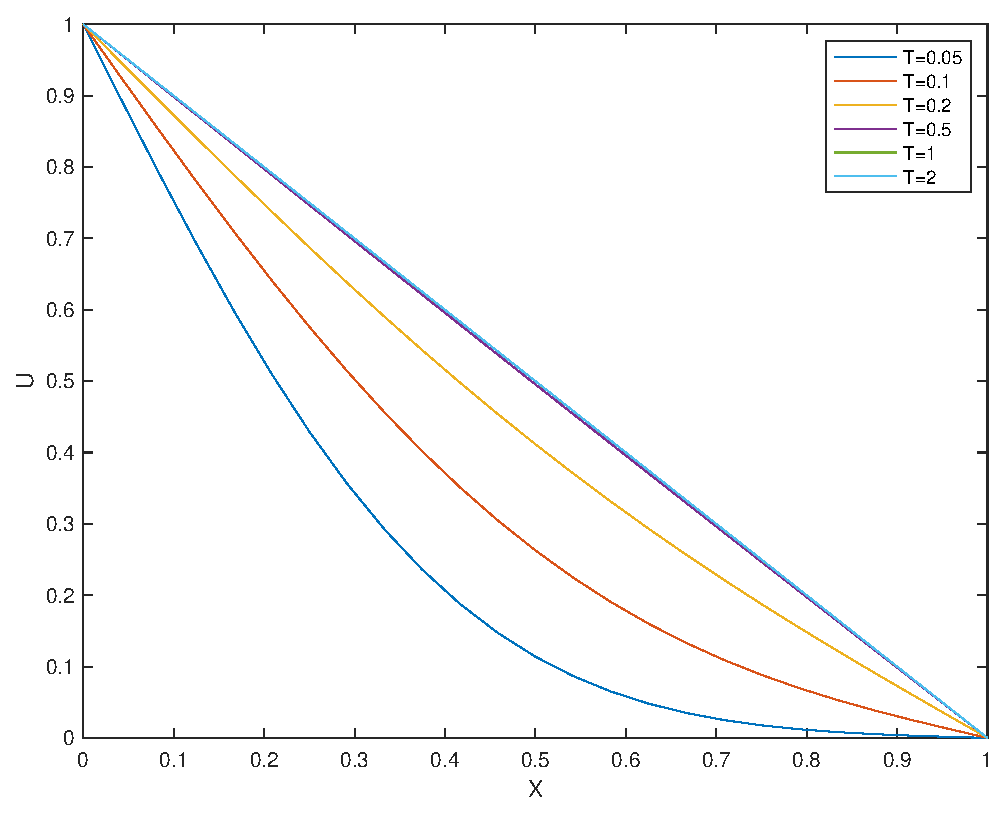
\includegraphics[width=10cm]{Image_2_1_1}
\caption{Solution \eqref{eq:Sol 1} plotted at different $T$}
\label{fg:ExactSol1}
\end{center}
\end{figure}

\begin{figure}[H]
\begin{center}
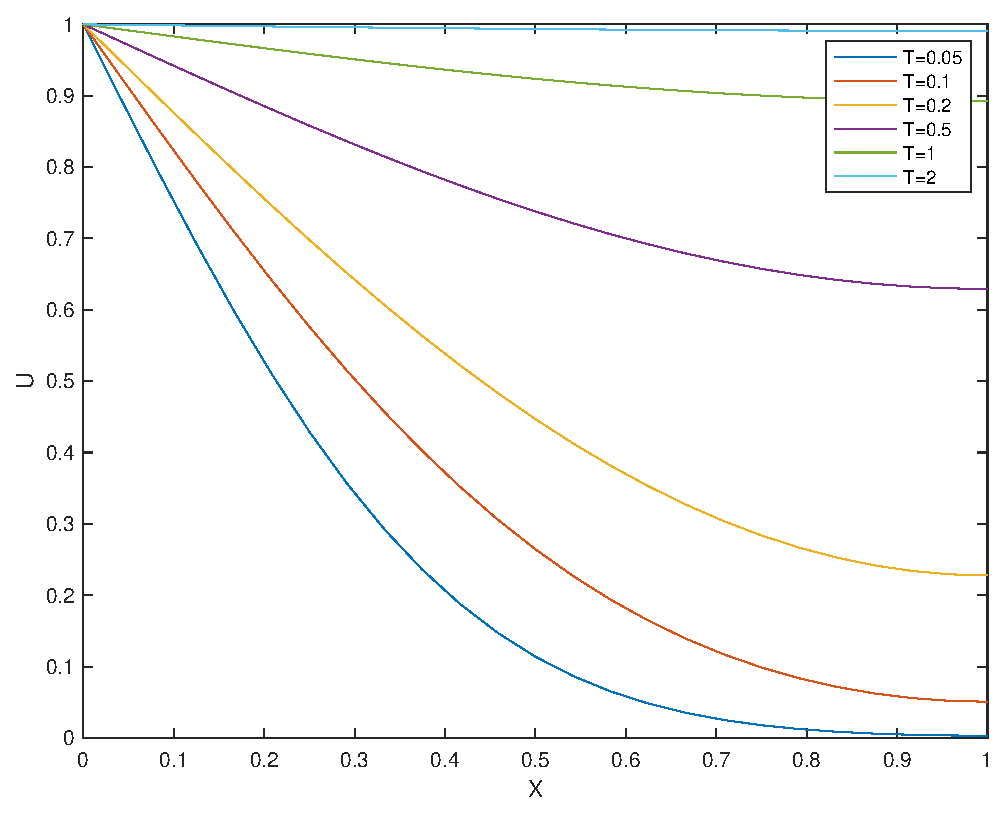
\includegraphics[width=10cm]{Image_2_1_2}
\caption{Solution \eqref{eq:Sol 2} plotted at different $T$}
\end{center}
\end{figure}

\begin{figure}[H]
\begin{center}
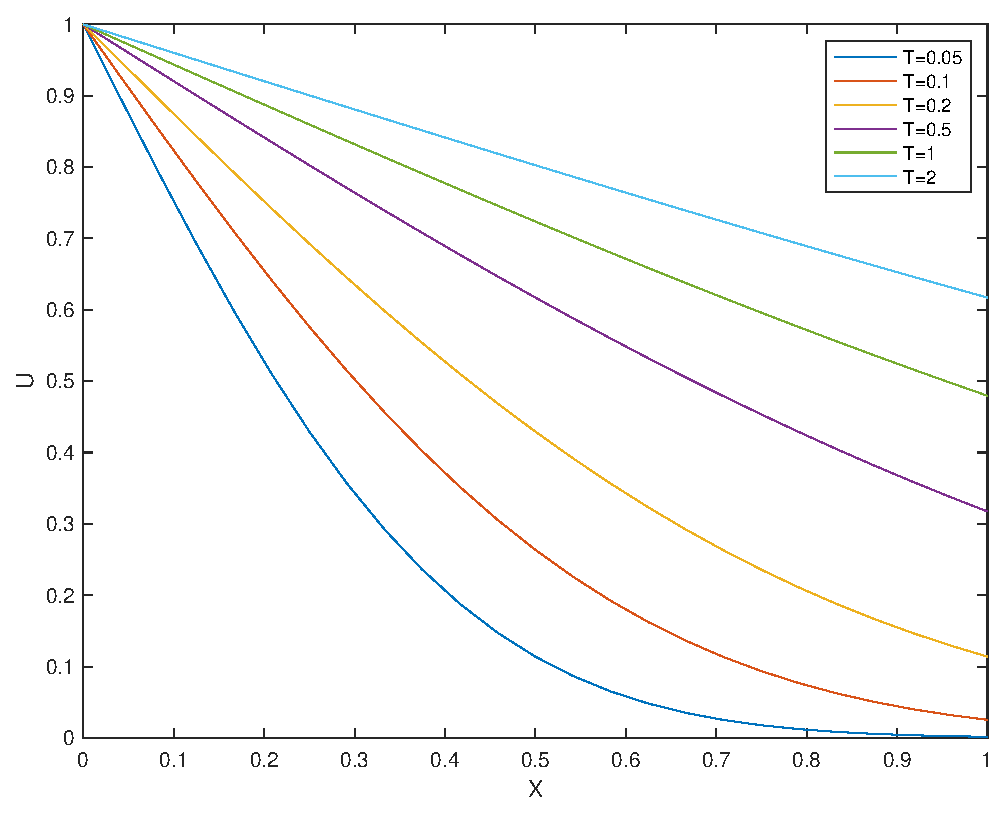
\includegraphics[width=10cm]{Image_2_1_3}
\caption{Infinite Solution plotted at different $T$}\label{fg:ExactSol2}
\end{center}
\end{figure}


As $T$ increases, the first two solutions tend towards the inhomogeneous functions $U_{s}(X)$ in Question 2. This is because the exponential part of homogeneous solution tends to zero sufficiently fast for the infinite sum to tend to zero. This makes sense, since intuitively the first solution will reach a symmetric equilibrium between 1 and 0, and the second solution will tend to the constant value 1.\\
The semi-infinite solution also tends towards the long time solution of equation \eqref{eq:Sol 2} but far slower. Again this makes sense; as heat dissipates along the bar it will reach (locally) a constant long time solution equal to the sourcing value 1. The reason it converges slower is because as $T\rightarrow \infty$, $\xi\rightarrow 0$, so Taylor expanding the exact solution gives
\begin{equation}
\erfc\left(\frac{1}{2}\xi\right)\approx 1-\frac{2\xi}{\sqrt{\pi}}+O\left(\xi^{2}\right)
\end{equation}
This equation tends to 1 with order $O\left(T^{-1/2}\right)$, which is far slower than the exponential decay of the first two solutions. \\

Although these solutions exactly solve equation (13) or equation (1), these are only approximations for the real world solution. In all three cases the value of $U(1/2,1/2c)$ (where $c$ is the speed of light) has increased from it's initial value of 0. If we assume the bar is 1m in length, this is not consistent with the laws of general relativity; heat cannot dissipate faster than the speed of light. Instead we expect the temperature at $X=1/2$ to remain equal to 0 until $T\geq 1/2c$.  Although this increase in $U(1/2,1/2c)$ is incredibly small and can be neglected, it is still greater than 0 and so we can conclude that these solutions are approximations. 

 \subsubsection*{\centering Heat Flux}\label{subsec:Heat Flux}
Calculating the heat flux $-U_{X}$ at $X=0$ for the three solutions gives
\begin{equation} \label{eq:HeatFlux}
\begin{aligned}
-U_{X} &= 1+2\sum_{n\geq 1}^{\infty}\exp\left(-\left(n\pi\right)^{2}T\right) \\
-U_{X} &= 2\sum_{n\geq 1}^{\infty}\exp\left(-\left(\frac{2n-1}{2}\pi\right)^{2}T\right) \\
-U_{X} &= \frac{1}{\sqrt{\pi KT}}
\end{aligned}
\end{equation}
(for equations \eqref{eq:Sol 1}, \eqref{eq:Sol 2} and the infinite solution (11) respectively).  \nameref{cd:2.1} was used to calculate and plot these functions in Figure \ref{fg:Heat Flux} (it is assumed that $K=1$). They were calculated to an accuracy of $0.5\times 10^{-5}$, which is again considered more generally in the subsection '\nameref{subsec:Truncated Error}' on page \pageref{subsec:Truncated Error}. 

\begin{figure}[H]
\centering
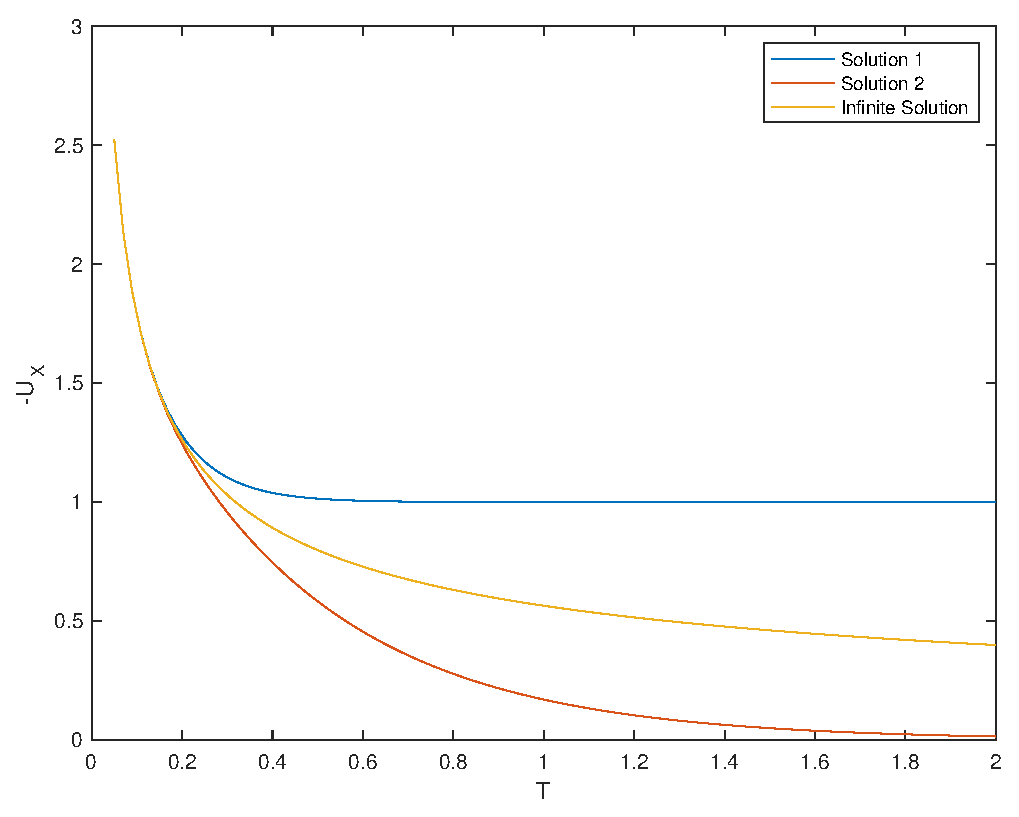
\includegraphics[width=10cm]{Image_2_7}
\caption{Heat Flux at $X=0$ for different $T$}\label{fg:Heat Flux}
\end{figure}
We can see that all the solutions diverge as $T\rightarrow 0$, which represents the fact that at $T=0$ we have a discontinuity at $X=0$, and all heat can travel to the right with no 'resistance'. \par
We can see that the first solution's heat flux tends to 1. This is because when the heat travels across the bar, it encounters the cooler end and so must continuously dissipate more and more heat from its source in order to maintain a steady state solution. The second solution tends to zero, as does the infinite solution, however the difference is that we expect
\begin{equation}
\int_{0}^{\infty}-U_{X}\mathrm{d}T
\end{equation}
to converge for solution 2 and not for the infinite solution. The above integral represents the energy flow across $X=0$ per unit cross sectional area. When the bar is finite (provided no heat is lost to the surroundings), a finite amount of energy must be required to heat this bar from the value 0 to 1, so only a finite flow of energy across this boundary is expected, whereas when the bar is infinite this is not the case and so the integral should diverge. Sure enough we deduce that $-\int_{0}^{\infty}U_{X}dT=\left[(2/\pi) \sqrt{\pi T}\right]_{0}^{\infty}\rightarrow \infty$ in the infinite bar case. When the bar is finite we have 
\begin{equation}\label{eq:HFShan}
\begin{aligned}
\int_{0}^{\infty}-U_{X}\mathrm{d}T &= 2\sum_{n\geq 1}^{\infty}\int_{0}^{\infty}\exp\left(-\left(\frac{2n-1}{2}\pi\right)^{2}T\right)\mathrm{d}T\\
&=2\sum_{n\geq 1}^{\infty}\left(\frac{2}{(2n-1)\pi}\right)^{2}\\
&= \frac{8}{\pi^2} \times \frac{3}{4} \times \frac{\pi^{2}}{6}\\
&= 1 \footnotetext{Hello}
\end{aligned}
\end{equation}
Therefore the total energy per unit area to heat the bar from 0 to 1 is 1.\footnote{In the derivation of equation \eqref{eq:HFShan} we use that $\sum_{n\geq 1}^{\infty}1/(2n-1)^{2}=3\pi^2/24$. This is because
\begin{equation}
\begin{aligned}
\frac{\pi^{2}}{6} &=\sum_{n \text{ odd}}1/n^2+\sum_{n \text{ even}}1/n^2 = \sum_{n \text{ odd}}1/n^2 + \sum_{n\geq 1}1/(2n)^2\\ 
&= \sum_{n \text{ odd}}1/n^2 + 1/4 \times \pi^2/6\\
\end{aligned}
\end{equation}
and hence the result follows.
} Since we are assuming $L=1$, we recover that in the non dimensional case of this problem,  the specific heat $\sigma =1$.

\subsubsection*{\centering Truncated Error}\label{subsec:Truncated Error}
In order to evaluate solution \eqref{eq:Sol 1} efficiently, we must find a lower bound for $k$ such that

\begin{equation} \label{eq:Small Error 1}
\sum_{n=k+1}^{\infty}\frac{2}{n\pi}\exp\left(-n^{2}\pi^{2}T\right)\abs{\sin\left(n\pi X\right)}
\end{equation}

is small.  We can find a lower bound for $A$ such that $A/n^{t}\geq \exp(-n^{2}\pi^{2}T)$ for all $n$ and $t$ is a positive number to be determined later.  Multiplying through by $n^{t}$ and finding the maximum of the right hand side gives

\begin{equation}
A=\exp\left(-\frac{t}{2}\right)\left(\frac{1}{\pi}\sqrt{\frac{t}{2T}}\right)^{t}
\end{equation}

and so equation \eqref{eq:Small Error 1} is less than or equal to
\begin{equation}\label{eq:Small Error 2}
\frac{2A}{\pi}\sum_{n=k+1}^{\infty}\frac{1}{n^{t+1}}\leq \frac{2A}{\pi}\int_{n=k}^{\infty}\frac{1}{n^{t+1}}\mathrm{d}n=\frac{2A}{\pi tk^{t}}
\end{equation}
(It is assumed that $k\geq 1$). If equation \eqref{eq:Small Error 2} is less than or equal to $\varepsilon$ then it is sufficient for $k\geq \left(2A/\pi t \varepsilon\right)^{1/t}$. Notice that this is true for any value of $t$, so we now aim to choose $t$ such that $k$ is minimised.  Differentiating the right hand side with respect to $t$ gives the equation $\ln\left(t\right)=1+\ln\left(2/\pi\varepsilon\right)-(1/2)t$. So $t=2W\left(e/\pi\varepsilon\right)$ where $W$ is the Lambert $W$ function and it is sufficient for
\begin{equation}\label{eq:KEq}
k\geq \max\left(\frac{1}{\pi}\sqrt{\frac{t}{2T}}\exp\left(-\frac{1}{t}\right) \, , \, 1\right)
\end{equation}
where $t$ is defined just above.
For solution \eqref{eq:Sol 2} notice that $n-1<\frac{2n-1}{2}<n$ so the truncated error is less than
\begin{equation}
\sum_{n=k+1}^{\infty}\frac{2}{\left(n-1\right)\pi}\exp\left(-\left(n-1\right)^{2}\pi^{2}T\right)
\end{equation}
Essentially this sum only includes one more term so it is sufficient to choose $k$ to be one greater than the previous case. This conclusion leads to some incredibly small values of $k$, if we require the solution to be accurate to 100 decimal places we only require 22 (or 23) terms in our series! Of course this is assuming that our computer can evaluate terms to an infinite precision, which it can't.\\

Notice that for a fixed $\varepsilon>0$, as $T\rightarrow\infty$, we may truncate earlier and earlier. This confirms what was observed in the first part of Question 2; that the solution $U(X,T)$ tends towards the inhomogeneous solution and the infinite series contributes less as $T$ grows. \\
When $T>0$, the lower bound for $k$ (equation \eqref{eq:KEq}) always exists and is independent of $x$, so we can conclude that, for any $T>0$, as $k\rightarrow\infty$ our truncated sum converges uniformly towards the analytic solution. When $T=0$ we deduce something different. By truncating our series at any point our approximation becomes continuous. Since it always passes through the point (0,1) we know that for any $\epsilon>0\,\,\,\exists\,\,\,\delta>0$ such that the approximation is greater than $\max\left(1-\epsilon,1/2\right)$ in the interval $[0,\delta]$. In particular our truncated sum only converges point wise, not uniformly, towards the analytic solution. (This is an application of the uniform limit theorem).\\

When plotting the heat flux using equation \eqref{eq:HeatFlux}, we want $2\sum_{k+1}^{\infty}\exp\left(-(n\pi)^{2}T\right)$ to be small. Following a similar method we deduce 
\begin{equation}
\begin{aligned}
2\sum_{n=k+1}^{\infty}\exp\left(-n^{2}\pi^{2}T\right) &\leq  2\int^{\infty}_{k}\exp\left(-\left(x\pi\sqrt{T}\right)^{2}\right)\mathrm{d}x\\ &\leq \frac{1}{k \pi^{2}T}\int_{k\pi\sqrt{T}}^{\infty}2u\exp\left(-u^{2}\right)\mathrm{d}u \\ &=\frac{1}{k\pi^{2}T}\exp\left(-k^{2}\pi^{2}T\right) \\ &\leq \frac{1}{\pi^{2}T}\exp\left(-k^{2}\pi^{2}T\right) \leq \varepsilon
\end{aligned}
\end{equation} 
(It is assumed that $k\geq 1$). Therefore we conclude it's sufficient for our sum to have error less than $\varepsilon$ when \begin{equation}
k\geq \max\left(\sqrt{\frac{-\log\left(\epsilon\pi^{2}T\right)}{\pi^{2}T}}\, ,\,1\right)
\end{equation}
The heat flux for solution \eqref{eq:Sol 2} only contains one extra term, so it is sufficient for our $k$ to be one greater than the $k$ in the previous case.\\ 


To preserve condition (16a) we require the gradient $U_{X}(1,T)=0$ for all $T$. Approximating the gradient at $X=1$ using the central difference method gives 
\begin{equation}
\frac{\partial U(X,T)}{\partial X}\approx\frac{U(X+\delta X,T)-U(X-\delta X,T)}{2\delta X}=\frac{U_{N+1}^{m}-U_{N-1}^{m}}{2\delta X}=0
\end{equation}
which forces $U_{N+1}^{m}=U_{N-1}^{m}$ for all $m$. \\

It makes sense to make $U_{0}^{0}$ the midpoint between the two conditions $\lim_{T\rightarrow 0}U(0,T)=1$ and $\lim_{X\rightarrow 0}U(X,0)=0$ in order for one condition to not outweigh the other. Running the program with different starting values of $0\leq U_{0}^{0}\leq 1$ actually doesn't affect the results greatly, it only increasing the error of the approximation slightly, and so we justify the choice that $U_{0}^{0}=0.5$ so that it minimises the error in our final solution.


\subsection*{\centering Question 3}
\nameref{cd:3.1} was used to tabulate the data in Tables \ref{tb:NumData1}-\ref{tb:NumData2}.\footnote{Note that the function \texttt{U2} was used implicitly in \nameref{cd:3.1} without it being referenced.} Since the values of $U\gtrsim 0.03$ (smallest value when $T=0.05$, we should set the error when calculating the analytic solution to be at most $5\times10^{-18}$, since MATLAB stores values to a precision of 16 significant figures.  This will ensure the error in the numerical scheme is calculated accurately. 

\begin{table}[H]
\centering
\begin{tabular}{|c|c|c|c|}
\hline $X_{n}$ & Numerical Solution & Analytic Solution & Error $E_{n}$ \\ \hline 0 & 1.0 & 1.0 & 0\\ 0.1 & 0.8238048553466797 & 0.8230821352256753 & 7.227201210043832e-4\\ 0.2 & 0.6556272506713867 & 0.6547769718120018 & 8.502788593849342e-4\\ 0.3 & 0.5034847259521484 & 0.5024786137685202 & 0.001006112183628227\\ 0.4 & 0.3714456558227539 & 0.3714399086227188 & 5.747200035099986e-6\\ 0.5 & 0.2635784149169922 & 0.26434868475581 & -7.702698388177831e-4\\ 0.6 & 0.1792669296264648 & 0.1814576074706133 & -0.002190677844148503\\ 0.7 & 0.1178951263427734 & 0.1211753009345904 & -0.003280174591816953\\ 0.8 & 0.07677221298217773 & 0.08092862782846388 & -0.004156414846286149\\ 0.9 & 0.0532073974609375 & 0.05807764171066454 & -0.00487024424972704\\ 1.0 & 0.04581451416015625 & 0.05069463731552959 & -0.004880123155373339\\ \hline \end{tabular}
\caption{$T=0.1$}\label{tb:NumData1}
\end{table}
\begin{table}[H]
\centering 
\begin{tabular}{|c|c|c|c|}\hline $X_{n}$ & Numerical Solution & Analytic Solution & Error $E_{n}$ \\ \hline 0 & 1.0 & 1.0 & 0\\ 0.1 & 0.8761711978968378 & 0.8761312670255909 & 3.99308712469848e-5\\ 0.2 & 0.7557321005760969 & 0.7557519398310537 & -1.98392549568549e-5\\ 0.3 & 0.6420724128201982 & 0.6421695686245892 & -9.715580439095817e-5\\ 0.4 & 0.5379536263039881 & 0.5383534783960334 & -3.998520920452941e-4\\ 0.5 & 0.4461372327023128 & 0.4468241081499145 & -6.868754476017092e-4\\ 0.6 & 0.3684343697768782 & 0.3695989288601486 & -0.0011645590832704\\ 0.7 & 0.3066561752893904 & 0.3081944368952941 & -0.001538261605903757\\ 0.8 & 0.2617214122328733 & 0.2636728148964549 & -0.001951402663581625\\ 0.9 & 0.2345488436003507 & 0.2367137602625006 & -0.002164916662149907\\ 1.0 & 0.225403107890088 & 0.2276883931414093 & -0.002285285251321323
 \\ \hline \end{tabular}
\caption{$T=0.2$}
\end{table}
\begin{table}[H]
\centering
\begin{tabular}{|c|c|c|c|}\hline $X_{n}$ & Numerical Solution & Analytic Solution & Error $E_{n}$ \\ \hline 0 & 1.0 & 1.0 & 0\\ 0.1 & 0.9420521555005696 & 0.9419937288524313 & 5.842664813837661e-5\\ 0.2 & 0.8855227491356883 & 0.8854163257976844 & 1.064233380039248e-4\\ 0.3 & 0.8318302190399054 & 0.8316613531229 & 1.688659170053786e-4\\ 0.4 & 0.7822538653514411 & 0.7820526575165497 & 2.012078348914148e-4\\ 0.5 & 0.7380729882085163 & 0.7378117244250572 & 2.612637834591425e-4\\ 0.6 & 0.700302471782793 & 0.700027610897948 & 2.74860884845074e-4\\ 0.7 & 0.6699572002459336 & 0.6696301951229767 & 3.270051229569138e-4\\ 0.8 & 0.64768852911673 & 0.6473673870072886 & 3.211421094414524e-4\\ 0.9 & 0.6341478139139741 & 0.6337868375726663 & 3.609763413078282e-4\\ 1.0 & 0.6295594452942082 & 0.6292225702004761 & 3.368750937320364e-4 \\ \hline \end{tabular}
\caption{$T=0.5$}
\end{table}
\begin{table}[H]
\centering
\begin{tabular}{|c|c|c|c|}\hline $X_{n}$ & Numerical Solution & Analytic Solution & Error $E_{n}$ \\ \hline 0 & 1.0 & 1.0 & 0\\ 0.1 & 0.9832113641530977 & 0.9831086687569828 & 1.026953961149601e-4\\ 0.2 & 0.9668335754721341 & 0.966633258156736 & 2.003173153981574e-4\\ 0.3 & 0.9512774811230473 & 0.9509794474936005 & 2.980336294468033e-4\\ 0.4 & 0.9369137116857988 & 0.9365326855414489 & 3.810261443499829e-4\\ 0.5 & 0.924112897740349 & 0.9236486995249148 & 4.641982154341973e-4\\ 0.6 & 0.9131691733766819 & 0.9126447359346814 & 5.244374420004805e-4\\ 0.7 & 0.9043766726847813 & 0.9037917488669897 & 5.849238177916272e-4\\ 0.8 & 0.8979242413728236 & 0.8973077282361593 & 6.165131366642207e-4\\ 0.9 & 0.8940007251489851 & 0.893352332141321 & 6.483930076640609e-4\\ 1.0 & 0.8926711958090956 & 0.892022955555891 & 6.482402532046461e-4 \\ \hline \end{tabular}
\caption{$T=1$}\label{tb:NumData2}
\end{table}
\begin{figure}[H]
\begin{center}
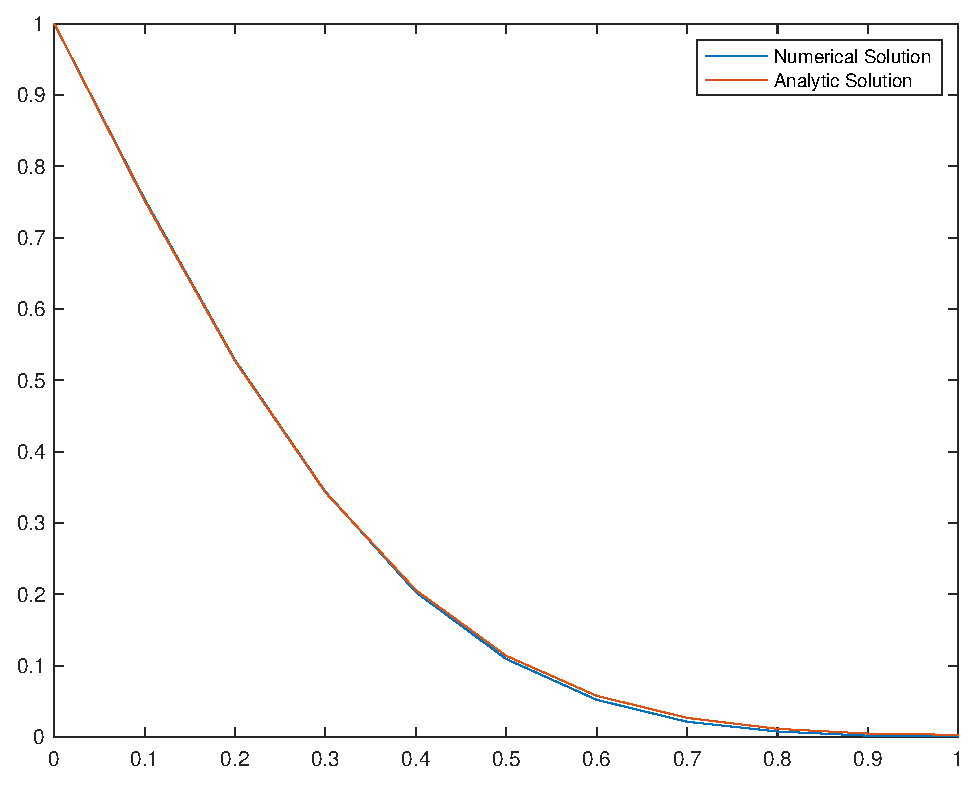
\includegraphics[width=10cm]{Image_3_1}
\caption{Numerical and analytic solution $T=0.05$}
\end{center}
\end{figure}
\begin{figure}[H]
\begin{center}
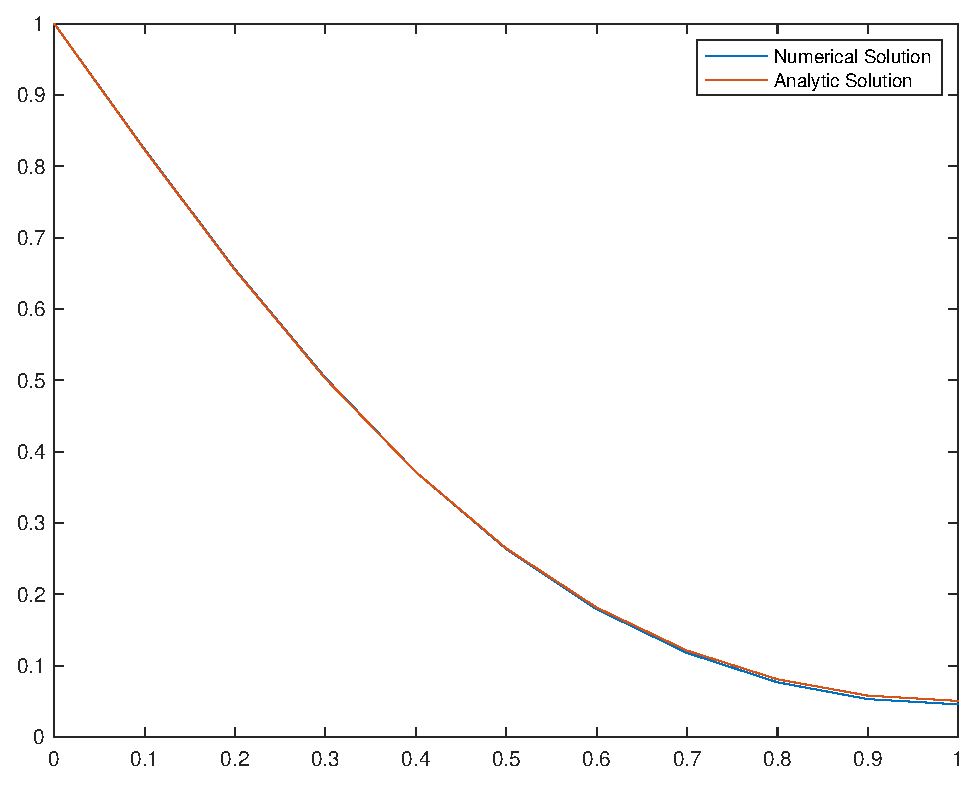
\includegraphics[width=10cm]{Image_3_2}
\caption{Numerical and analytic solution $T=0.1$}
\end{center}
\end{figure}
\begin{figure}[H]
\begin{center}
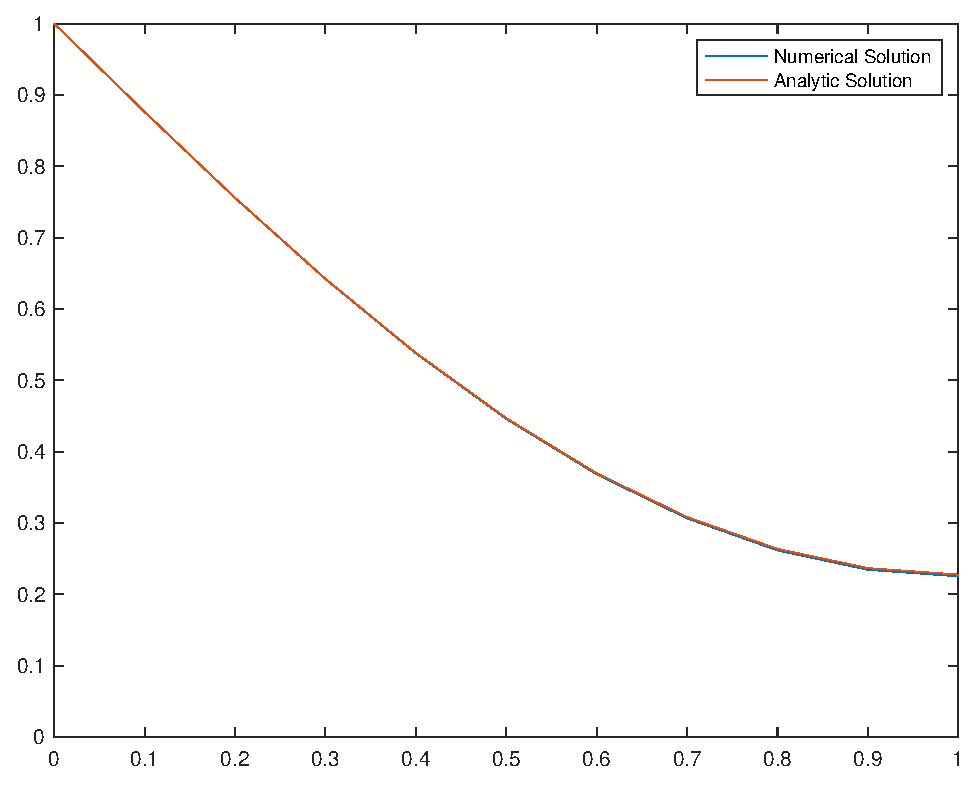
\includegraphics[width=10cm]{Image_3_3}
\caption{Numerical and analytic solution $T=0.2$}
\end{center}
\end{figure}
\begin{figure}[H]
\begin{center}
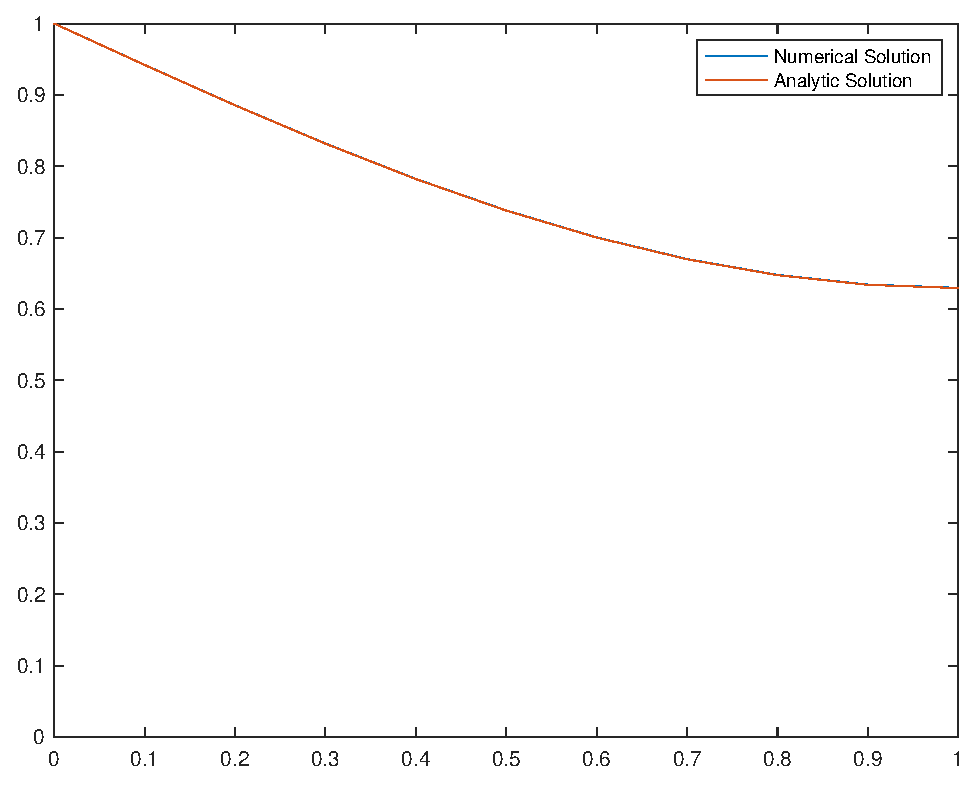
\includegraphics[width=10cm]{Image_3_4}
\caption{Numerical and analytic solution $T=0.5$}
\end{center}
\end{figure}
\begin{figure}[H]
\begin{center}
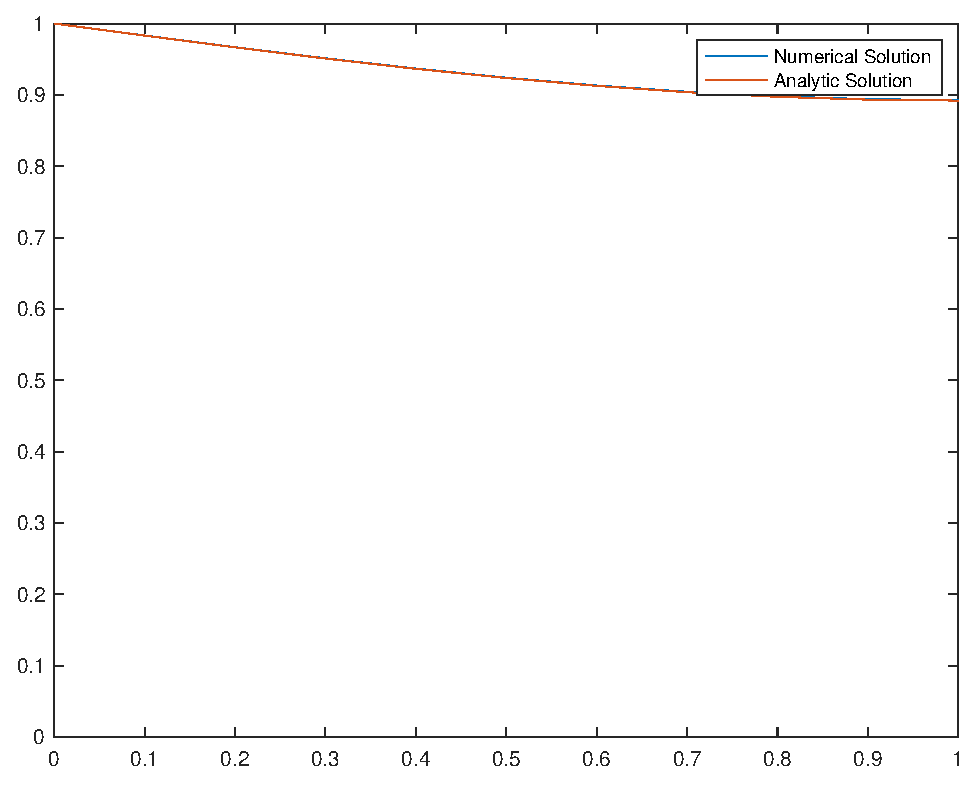
\includegraphics[width=10cm]{Image_3_5}
\caption{Numerical and analytic solution $T=1.0$}
\end{center}
\end{figure}
\begin{figure}[H]
\begin{center}
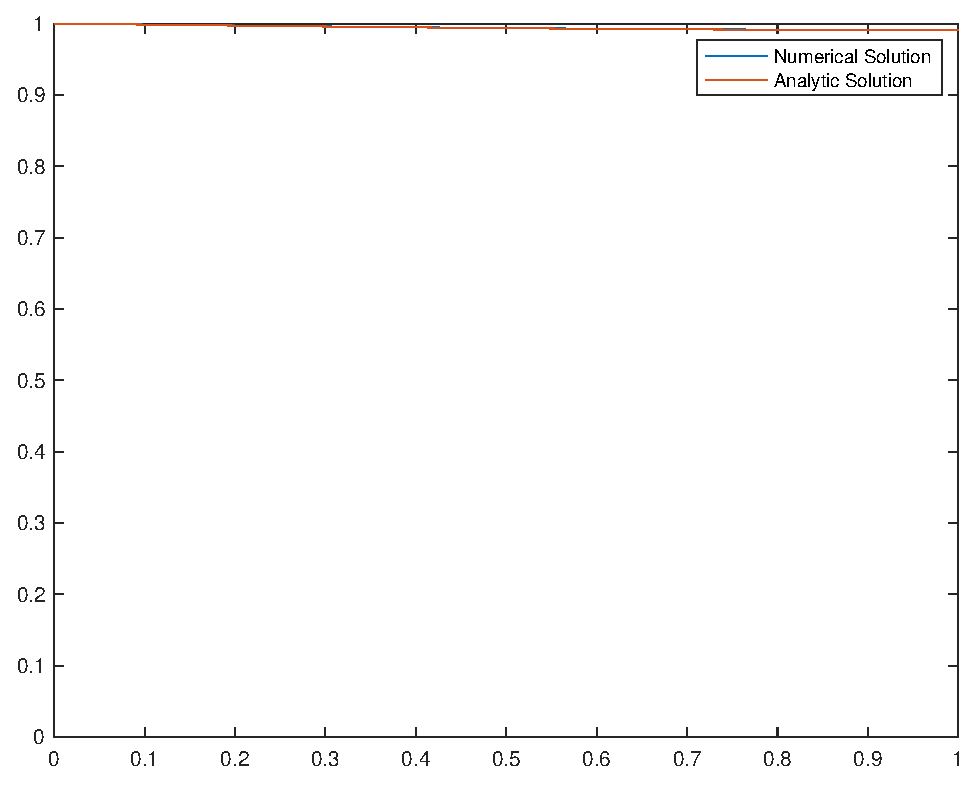
\includegraphics[width=10cm]{Image_3_6}
\caption{Numerical and analytic solution $T=2.0$}
\end{center}
\end{figure}
It's clear that this numerical approximation is very close to the analytic solution. Note that as $X$ increases from 0 to 1, the error in the approximation seems to increase (column 4 of Tables \ref{tb:NumData1} to \ref{tb:NumData2}). This makes intuitive sense, since with each iteration as $X$ increases, our scheme will use already erroneous data to forecast $U(X+\delta X,T$), so we expect the error to grow. Also notice that the error seems to tend to some constant value as $X$ increases. This is caused by  imposing the condition that our numerical solution has gradient 0 at $X=1$, and so the error must stabilise. The accuracy and stability of this method will now be discussed in greater detail in the following two subsections.
\subsubsection*{\centering Order of Accuracy}
We aim to find an upper bound on the error of this numerical scheme. The absolute error $\epsilon_{n}^{m}$, when evaluating $U_{n}^{m}$, satisfies the difference equation
\begin{equation}\label{eq:SpecialC}
\epsilon_{n}^{m+1}=\epsilon_{n}^{m}+C\left(\epsilon_{n+1}^{m}-2\epsilon_{n}^{m}+\epsilon_{n-1}^{m}\right)+O\left(\left(\delta T\right)^{2}\right)+O\left(\delta T \left(\delta X\right)^{2}\right)
\end{equation} 
When $C\leq 1/2$, we may take the maximum over $n$ (since all the coefficients of the equation are positive) to give
\begin{equation}
\epsilon^{m+1} \leq \epsilon^{m} +A\left(\left(\delta T\right)^{2}+\delta T \left(\delta X\right)^{2}\right)
\end{equation}
where $\epsilon^{m}=\max_{n=0,1,...,N}\left(\epsilon_{n}^{m}\right)$ and $A$ is some constant determined by the maximum of the higher derivatives of $U$ (we are assuming these are continuous and hence bounded). Using the fact that $\epsilon^{0}=0$, we deduce (by induction) that
\begin{equation}
\begin{aligned}
\epsilon^{m} &\leq Am\left(\left(\delta T\right)^{2}+\delta T \left(\delta X\right)^{2}\right)\\
&\leq AT\left(\delta T+\left(\delta X\right)^{2}\right)\\
&= AT\left(1+\frac{1}{C}\right)\delta T\\
&= AT\left( 1+C\right)\left(\delta X\right)^{2}
\end{aligned}
\end{equation}
This numerical scheme therefore converges to the solution for all $C\leq 1/2$ as $\delta T$ and $\delta X$ tend to 0.\footnote{This method was motivated by the methods in \cite{AMES199250}} For a fixed value of $C$, it is also first order accurate in $\delta T$, or second order accurate in $\delta X$. 
Confirming this idea, \nameref{cd:3.2} referenced on page \pageref{cd:3.2} calculated the error when approximating $U(1,0.1)$ for different values of $\delta X$, while $C=1/2$.\footnote{Note that the functions \texttt{U2} and \texttt{numU} were used implicitly in \nameref{cd:3.2} without being referenced.} This data is presented in Table \ref{tb:accurateerror}. 
\begin{table}[H]
\centering
\begin{tabular}{|c|c|} \hline $\delta X_{n}$ & Error at $U(1,0.1)$\\ \hline 0.1 & 0.0048801231553733\\ 0.05 & 0.0012204864884093\\ 0.025 & 0.00030511086347493\\ 0.0125 & 7.6276428956995e-5\\ 0.00625 & 1.9069017255853e-5\\ 0.003125 & 4.7672485409267e-6\\ 0.0015625 & 1.1918117721055e-6\\ 0.00078125 & 2.9795292000312e-7 \\ \hline
\end{tabular}
\caption{Error in $U(0,0.1)$ for different values of $\delta X$}
\label{tb:accurateerror}
\end{table}
Plotting this data in Figure \ref{fg:AccurateError1} below on a log log axis and calculating the least squares regression line gives the gradient of $S_{XY}/S_{XX}=1.99996839724059\approx 2$.  This confirms that this is a second order method. This is because if the error $\epsilon\left(h\right)\approx A\times h^{n}$, e.g was $n$-th order in step size $h$, then $\log\left(\epsilon\right)=B+n\log\left(h\right)$ for constants $A$ and $B$. Hence plotting $\log\left(\epsilon\right)$ against $\log\left(h\right)$ would give a straight line of gradient $n$; in this case 2. 
\begin{figure}[H]
\centering
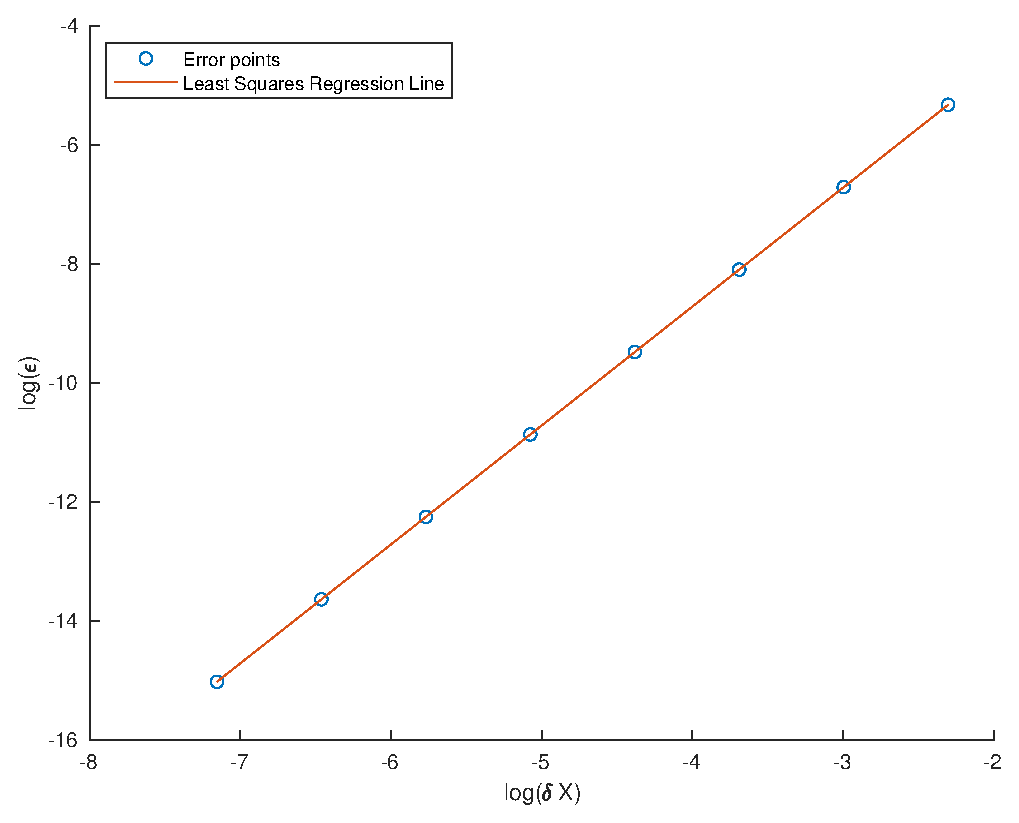
\includegraphics[width=10cm]{Image_3_1_Order_Of_Accuracy}
\caption{$\log\left(E_{n}\right)$ against $\log\left(\delta X_{n}\right)$}
\label{fg:AccurateError1}
\end{figure}
This also confirms that this method is first order in $\delta T$, since if $C$ is constant, then $\left(\delta X\right)^{2} \propto \delta T$, therefore $\epsilon\left(\delta T\right)\propto A \left(\sqrt{\delta T}\right)^{2}$ which is first order.\\

We now investigate the accuracy of the method for different values of $C$.
Calculating the error in $U(1,1)$ for $N=10$ yields Table \ref{tb:C error} below (produced by Code 3.1).
\begin{table}[H]
\centering
\begin{tabular}{|c|c|}
\hline
$C$ & Error in $U(1,1)$    \\ \hline
1 & 5.88453360765802e+44 \\
1/2                      & 0.000648240253204646 \\
1/4                      & 0.000162686626762443 \\
1/5                      & 6.49296577892589e-05 \\
1/10                     & 0.000130407637938257 \\
1/20                     & 0.000227988118626898 \\ \hline
\end{tabular}
\caption{Error in $U(1,1)$ with $N=10$, and different $C$}\label{tb:C error}
\end{table}
When $C=1$ our method is unstable, however this is discussed in greater detail in the section '\nameref{subsec:StabSol}' on page \pageref{subsec:StabSol}. What is interesting is the error initially decreases as $C$ decreases, however after some point it begins to increase, implying there may be some optimal value of $C$ such that this method converges the fastest.  This turns out to be true, with this 'special' value of $C$ equalling 1/6. \par
This is because if we were to expand the first line of working of equation \eqref{eq:SpecialC}, so that we included terms of order $\left(\delta T\right)^{2}$ and $\left(\delta X\right)^{2}$, we would include the terms
\begin{equation}
\hdots - \frac{1}{2}\frac{\partial^{2} U}{\partial T^{2}}\left(\delta T\right)^{2} +\frac{1}{12}\frac{\partial^{4} U}{\partial X^{4}}\delta T\left(\delta X\right)^{2} +O\left(\left(\delta T\right)^{3}+\delta T\left(\delta X\right)^{4}\right)
\end{equation}
However using equation (13) and interchanging the order of mixed partial derivatives, $
\partial^{2}U/\partial T^{2}=\partial^{4}U/\partial X^{4}$, so the above two terms would cancel if $\delta T/\left(\delta X\right)^{2}=C=1/6$. If this is the case, this numerical scheme becomes 2nd order in $\delta T$ or 4th order in $\delta X$, and hence the error in $U(1,1)$ decreases faster.

\subsubsection*{\centering Stability of Solution}\label{subsec:StabSol}
We saw earlier that for any $C\leq1/2$ this method converges to the solution. We will find that for any $C> 1/2$ this method is unstable.\\
Note that whenever $C$ is an integer, the values of $U_{n}^{m}$ can only take the form $p+(1/2)q$ where $p, q\in \Z$. This follows by a simple induction on equation (21). It is therefore impossible for $U_{n}^{m}$ to have an arbitrarily small error, and hence this method will never converge. Below is Figure \ref{fg:Div1} that portrays this for $C=1, T=1$ and $N=10$.
\begin{figure}[H]
\centering
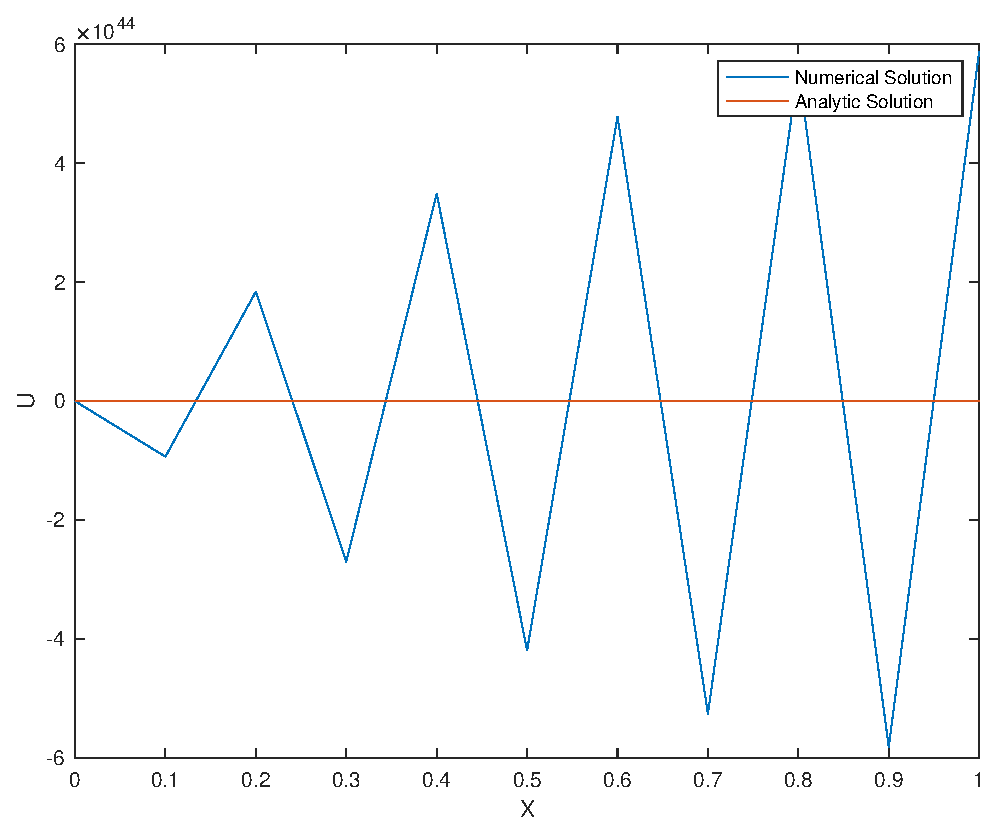
\includegraphics[width=10cm]{Image_3_1Wild}
\caption{Instability of method when $C$ is an integer}
\label{fg:Div1}
\end{figure}

The proof that this method diverges for $C>1/2$ is involved, however it is sketched out below:\\

Suppose the error of this method at the point $(X,T)$ could be expanded as a Fourier series;
\begin{equation}\label{eq:FourierTrans}
\epsilon\left(X,T\right)=\sum_{k=-K}^{K}E_{k}\left(T\right)e^{a_{k}\mathbf{i}X}
\end{equation}
where $K=1/\delta X$, $a_{k}=\pi k$ and $\mathbf{i}=\sqrt{-1}$. This assumes that the amplitude of the error $E_{k}$ is just a function of time. Since equation \eqref{eq:SpecialC} is linear (ignoring higher order terms), it suffices to investigate how one of the terms in equation \eqref{eq:FourierTrans} behaves. Substituting $\epsilon_{n}^{m}=E_{k}\left(m\delta T\right)e^{a_{k} \mathbf{i} n\delta X}$ into the difference equation leads to 
\begin{equation}
E_{k}\left(mT+\delta T\right)e^{a_{k}\mathbf{i}n\delta X} = E_{k}\left(mT\right)\left(Ce^{a_{k}\mathbf{i}(n+1)\delta X}+ Ce^{a_{k}\mathbf{i}(n-1)\delta X}+(1-2C)e^{a_{k}\mathbf{i}n\delta X}\right)
\end{equation}
or
\begin{equation}
\frac{E_{k}\left(m\delta T+\delta T\right)}{E_{k}\left(m\delta T\right)} = 1+C\left(\exp\left(a_{k}\mathbf{i}\delta X\right)+\exp\left(-a_{k}\mathbf{i} \delta X\right) -2\right)
\end{equation}
If we let $\theta = a_{k}\delta X$, then the above equals $1-4C\sin^{2}\left(\theta/2\right)$. A necessary condition for the error to remain bounded is for the modulus of this 'amplification factor' of $E_{k}$ to be less than or equal to 1 for all $\theta$.  In other words $C\leq 1/2$. Therefore we conclude that this method diverges for $C>1/2$.\footnote{This proof was motivated by the one laid out in Chapter 3.5 of \cite{trefethen1996finite}} This agrees with the Courant–Friedrichs–Lewy condition; that a necessary condition for the convergence of an explicit time integration scheme is that the Courant number $C$ must be less than a particular value. The reasoning for this is if the wave solution to the problem propagates too quickly between adjacent time steps such that the wave passes two adjacent space steps, then we will lose information about the wave and the results from this method will be incorrect.

Note that when $C>>1/2$, the amplification factor is less than -1 for almost all values of $\theta$. This means that for large $C$ this method will never monotonically diverge, instead it will oscillate. This is consistent with Figure \ref{fg:Div1} but not consistent when $C=0.501$. Table \ref{tb:NonOsc} below presents the exact error for this case, and it can be seen that it is not oscillating. (Table produced by Code 3.1)
\begin{table}[H]
\centering
\begin{tabular}{|c|c|}
\hline $X_{i}$ & Exact Error \\ \hline 0 & 0\\ 0.1 & -2.429543737858531e-5\\ 0.2 & -4.412813080534317e-5\\ 0.3 & -7.050812233944104e-5\\ 0.4 & -8.393672321749257e-5\\ 0.5 & -1.098190177734049e-4\\ 0.6 & -1.155290402048426e-4\\ 0.7 & -1.383800889013242e-4\\ 0.8 & -1.358125814520106e-4\\ 0.9 & -1.533955469568138e-4\\ 1.0 & -1.428018187988878e-4\\ \hline
\end{tabular}
\caption{Monotonic error when $C=0.501$}
\label{tb:NonOsc}
\end{table}

\section*{\centering References}\label{References}
\printbibliography[heading=none]

\pagebreak
\section*{\centering Code}
\subsection*{\centering Code 2.1}\label{cd:2.1}
\begin{verbatim}
format long

%This calculates the exact solutions at T=0.25 and X=0.125n
solutions=zeros(9,4);
counter=0;
while counter<=8
    solutions(counter+1,1)=0.125*counter;
    solutions(counter+1,2)=U1(0.125*counter,0.25,0.5*10^(-5));
    solutions(counter+1,3)=U2(0.125*counter,0.25,0.5*10^(-5));
    solutions(counter+1,4)=erfc(0.125*counter);
    counter=counter+1;
end
disp(solutions)
latex(sym(vpa(solutions)))

%This calculates the numerical values of solutions as they evolve in time
XPoints=25;
T=[0.05 0.1 0.2 0.5 1 2];
dimT=size(T,2);

Sol1=zeros(XPoints,dimT);
Sol2=zeros(XPoints,dimT);
InfSol=zeros(XPoints,dimT);
Counter=1;
while Counter<=dimT
    t=T(Counter);
    counter=0;
    while counter<=XPoints-1
        Sol1(counter+1,Counter+1)=U1((1/(XPoints-1))*counter,t,0.5*10^(-5));
        Sol2(counter+1,Counter+1)=U2((1/(XPoints-1))*counter,t,0.5*10^(-5));
        InfSol(counter+1,Counter+1)=erfc((1/(XPoints-1))*counter/(2*sqrt(t)));
        counter=counter+1;
    end
    Counter=Counter+1;
end
Sol1(:,1)=linspace(0,1,XPoints);
Sol2(:,1)=Sol1(:,1);
InfSol(:,1)=Sol1(:,1);

%This plots the 3 solutions
Counter=1;
figure
Legend=cell(dimT,1);
for iter=1:dimT
    Legend{iter}=strcat('T=',num2str(T(iter)));
end

while Counter<= dimT
    plot(Sol1(:,1),Sol1(:,Counter+1))
    hold on
    Counter=Counter+1;
end
legend(Legend)
xlabel('X')
ylabel('U')
print('Image_2_1','-depsc')

Counter=1;
figure
while Counter<= dimT
    plot(Sol2(:,1),Sol2(:,Counter+1))
    hold on
    Counter=Counter+1;
end
legend(Legend)
xlabel('X')
ylabel('U')
print('Image_2_2','-depsc')

Counter=1;
figure
while Counter<= dimT
    plot(InfSol(:,1),InfSol(:,Counter+1))
    hold on
    Counter=Counter+1;
end
legend(Legend)
xlabel('X')
ylabel('U')
print('Image_2_3','-depsc')



%HEAT FLUX
%Calculating the heat flux
epsilon=0.5*10^(-5);
T=linspace(0.05,2);
Counter=1;
Flux=zeros(100,4);
Flux(:,1)=T;
while Counter<=100
    k=ceil(sqrt(-log(epsilon*pi^2*T(Counter))/(pi^2*T(Counter))));
    n=k;
    Flux1=0;
    Flux2=exp(-((2*n+1)/2)^2*pi^2*T(Counter));
    while n>=1
        Flux1=Flux1+exp(-n^2*pi^2*T(Counter));
        Flux2=Flux2+exp(-((2*n-1)/2)^2*pi^2*T(Counter));
        n=n-1;
    end
    Flux1=2*Flux1+1;
    Flux2=2*Flux2;
    Flux(Counter,2)=Flux1;
    Flux(Counter,3)=Flux2;
    Flux(Counter,4)=1/sqrt(pi*T(Counter));
    Counter=Counter+1;
end
%Plots the heat flux
figure
plot(Flux(:,1),Flux(:,2:4))
legend('Solution 1','Solution 2','Infinite Solution')
xlabel('T')
ylabel('-U_X')
print('Image_2_7','-depsc')

%This calculates the first solution at X,T with error at most epsilon
function answer = U1(X,T,epsilon)
    answer=0;
    t=2*lambertw(exp(1)/(pi*epsilon));
    k=ceil((1/(pi))*exp(-1/t)*(sqrt(t/(2*T))));
    n=k;
        while n>=1
        g=-2/(n*pi)*exp((-(n*pi)^2)*T);
        h=sin(n*pi*X);
        answer=answer+g*h;
        n=n-1;
        end
    answer=answer+1-X;
end

%This calculates the second solution at X,T with error at most epsilon
function answer = U2(X,T,epsilon)
    answer=0;
    t=2*lambertw(exp(1)/(pi*epsilon));
    k=1+ceil((1/(pi))*exp(-1/t)*(sqrt(t/(2*T))));
    n=k;
        while n>=1
        g=-4/((2*n-1)*pi)*exp((-((2*n-1)*pi/2)^2)*T);
        h=sin((2*n-1)*pi*X/2);
        answer=answer+g*h;
        n=n-1;
        end
    answer=answer+1;
end
\end{verbatim}
\pagebreak
\subsection*{\centering Code 3.1}\label{cd:3.1}
\begin{verbatim}
format long g
T=0.05;
N=10;
C=0.5;

Counter=1;
Data=zeros(N+1,4);
Data(:,2)=numU(T,N,C);
while Counter<=N+1
    Data(Counter,1)=(Counter-1)/N;
    Data(Counter,3)=U2(Data(Counter,1),T,5*10^(-18));
    Data(Counter,4)=Data(Counter,2)-Data(Counter,3);
    Counter=Counter+1;
end

disp(Data)
latex(sym(vpa(Data)))

figure
plot(Data(:,1),Data(:,2))
hold on
plot(Data(:,1),Data(:,3))
legend('Numerical Solution','Analytic Solution','Location','northeast')
xlabel('X')
ylabel('U')
print('Image_3_1','-depsc')

%This calculates the numerical approximation to U at time T
function answer = numU(T,N,C)
    DeltaT=C/N^2;
    U=zeros(N+1,floor(T/DeltaT+1));
    U(1,:)=1;
    U(1,1)=0.5;
    ColCount=2;
    while ColCount<=T/DeltaT+1
        RowCount=2;
        while RowCount<=N
            U(RowCount,ColCount)=U(RowCount,ColCount-1)+...
                C*(U(RowCount-1,ColCount-1)-2*U(RowCount,ColCount-1)+...
                U(RowCount+1,ColCount-1));
            RowCount=RowCount+1;
        end
        U(RowCount,ColCount)=U(RowCount,ColCount-1)+2*C*(U(RowCount-1,...
            ColCount-1)-U(RowCount,ColCount-1));
        ColCount=ColCount+1;
    end
    answer=U(:,end);
end
\end{verbatim}
\pagebreak
\subsection*{\centering Code 3.2}\label{cd:3.2}
\begin{verbatim}
format long g
T=0.1;
N=10;
C=1/2;

%Calculates error for 8 points
W=U2(1,T,0.5*10^(-18));
Counter=0;
Points=zeros(8,2);
while Counter<=7
    Points(Counter+1,1)=1/(N*2^(Counter));
    V=numU(T,N*2^(Counter),C);
    Points(Counter+1,2)=abs(V(end,1)-W);
    Counter=Counter+1;
end
disp(Points)
digits(14)
latex(vpa(sym(Points)))
Points=log(Points);

%Calculates least squares regression line
SXX=dot(Points(:,1),Points(:,1))-(sum(Points(:,1)))^2/8;
SYY=dot(Points(:,2),Points(:,2))-(sum(Points(:,2)))^2/8;
SXY=dot(Points(:,1),Points(:,2))-sum(Points(:,1))*sum(Points(:,2))/8;
YMean=sum(Points(:,2))/8;
XMean=sum(Points(:,1))/8;
PMCC=SXY/(sqrt(SXX*SYY));

X=linspace(Points(1,1),Points(end,1));
Y=(SXY/SXX).*(X-XMean)+YMean;

%Plots scatter plot
figure
scatter(Points(:,1),Points(:,2))
hold on
plot(X,Y)
legend('Error points','Least Squares Regression Line','Location','northwest')
xlabel('log(\delta X)')
ylabel('log(\epsilon)')
print('Image_3_1_Order_Of_Accuracy','-depsc')

disp(SXY/SXX)
\end{verbatim}
\end{document}
